\documentclass[11pt, a4paper]{report}

\usepackage[utf8]{inputenc}
\usepackage{graphicx}
\usepackage{geometry, float}
\usepackage[style=authoryear, backend=biber]{biblatex}
\usepackage{mhchem}
\usepackage{amsmath}
\usepackage{pgfgantt}
\usepackage{titlesec}

\usepackage{listings}
\usepackage{xcolor}

% tables
\usepackage{booktabs}
\usepackage{ltablex}
\usepackage{array}
\usepackage{caption}

\geometry{ a4paper, margin=2cm, heightrounded}
\renewcommand{\baselinestretch}{1.15}
\setlength{\parindent}{0pt}
\setlength{\parskip}{0.8em}

% % Remove chapter from title
\titleformat{\chapter}[block]
  {\normalfont\huge\bfseries}
{\thechapter\quad}{0pt}{\Huge}

\addbibresource{references.bib}
\graphicspath{{images/}{figures/}}

% Row style in tables
\newcolumntype{+}{>{\global\let\currentrowstyle\relax}} % Start column style
\newcolumntype{^}{>{\currentrowstyle}} % Each subsequent column style
\newcommand{\rowstyle}[1]{\gdef\currentrowstyle{#1}#1\ignorespaces} % Set row style

% Figure References
\newcommand{\figref}[1]{Figure~\ref{#1}}

% Word Count
\newcommand{\wordcount}{
    \immediate\write18{texcount -1 -sum -merge dissertation.tex > dissertation_words.count}
    \input{dissertation_words.count}
}



\lstdefinestyle{mystyle}{
  basicstyle=\ttfamily\small,
  numbers=left,
  numberstyle=\tiny\color{gray},
  keywordstyle=\color{blue},
  commentstyle=\color{teal},
  stringstyle=\color{orange},
  breaklines=true,
}
\lstset{style=mystyle}


% Table of Contents
\renewcommand{\contentsname}{Table of Contents} % Change table of contents name

\begin{document}
\begin{titlepage}
    \centering

    
\includegraphics[width=0.75\textwidth]{newcastle_uni_logo.png}

    \vspace{2cm}

    {\large BSc (Hons) Computer Science}

    \vspace{2cm}

    {\huge\bfseries Comparing knowledge tracing algorithms on large language model synthesized students}

    \vspace{2cm}

    {\large
        Author: Jakub Watson-Jones\par
        Supervisor: Dr Huizhi Liang\par
        6 May 2026
    }

    \vfill
    Word count:
    \wordcount{}

\end{titlepage}


\chapter*{Abstract}
This dissertation looks at synthesizing user data for comparing knowledge tracing algorithms. The user synthesis scrip keeps track of an internal state and response history which is passed to a large language model. The large language model uses the user state to create realistic answers including mistakes. These answers are fed into a knowledge tracing model which tries to predict the correctness.

Collecting user data is difficult in GDPR restricted countries especially when the data concerns children learning simple mathematical operations.

\chapter*{Declaration}
I declare that this dissertation represents my own work except where stated otherwise.

\chapter*{Acknowledgements}
Firstly, I would like to thank my project supervisor Huizhi Liang for taking on my personal personal project. I'm grateful for her help with organizing the project, her helpful advice and for pushing me to do my best.



\tableofcontents

\chapter{Introduction}
\section{Context}
Maths education is a crucial part of everyone's lives. Its primary goal is to equip students with fluency in the fundamentals of mathematics, mathematical reasoning, and problem-solving, and to apply mathematical concepts in science and other fields~\parencite{Math_Curriculum_England}. Government reports suggest that the average class size is around 26.2 pupils~\parencite{Class_Size_England} and has an average pupil-teacher ratio of 18.0~\parencite{Pupil_Teacher_Ratio_England}. This high ratio inevitably limits the attention a teacher can provide to each student.

Learning is separated into two groups: procedural fluency and contextual understanding. In maths, there is a large emphasis on procedural fluency in the early stages of education. In the UK, pupils do mental arithmetic in Key Stage 1. This is why calculators are only introduced at the end of Key Stage 2~\parencite{Math_Curriculum_England}.

\section{Problem}
This section discusses the multiple problems addressed by the dissertation.

\subsection{Limitations of Static Pedagogical Models}
Teaching early arithmetic like addition, subtraction, multiplication and division requires a lot of practice. The large volume of practice required for effective procedural fluency results in a one size fits all solution of large lists of exercises. However, this static approach is suboptimal as a pupil can be given a previously mastered exercise that wastes their time or they mey encounter problems that they are unable to solve. The ideal balance of difficulty of exercise is known as the Zone of Proximal development~\parencite{Zone_of_Proximal_Development}.

The efficiency of practice can be automatized. Automatic adjustment of difficulty is only possible if there is an algorithm that a models the mastery of a student. These models are known as knowledge tracing models.

\subsection{Data sensitivity}
The target of learning simple arithmetic are children, which makes the collection of data a challenge. Specifically, the General Data Protection Regulation complicates the collection of training and testing data. To avoid this problem the training and comparison data will be synthesize.

\section{Aim and objectives}

The aim of this dissertation is to create an smart tutor artefact that estimates the user's mastery using knowledge tracing algorithms and create a user synthesis script. The knowledge tracing models will be train, tested and compared on the synthesized data. Finally the synthesized data will be compared to a publicly available dataset ASSISTments2009~\parencite{assist2009}. The artefact will have a user interface allowing real user interaction.

There are many knowledge tracing algorithms so this dissertation will use a subset of Deep Knowledge tracing algorithms implemented in the python library pyKT~\parencite{pyktPaper}. The specific algorithms are in alphabetical order: AKT, DKT, DTransformer, SAKT, and SimpleKT\@. These were selected to represent a range of cutting edge algorithms currently relevant in the field of knowledge tracing.

The artifact will generate synthetic user data, which will be used to train and test these knowledge tracing algorithms. The user synthesis script will keep track of a student state. This student state and the response history will be fed into a large language model to create a realistic response. This response will be used to update the student state.

\chapter{Background Research}
This section shows the research for this dissertation.

\section{Python Deep-Learning Knowledge Tracing library (pyKT)}
The pyKT library~\parencite{pyktPaper} implements a large number of modern knowledge tracing models. It provides a unified API to implement multiple algorithms and datasets enabling comparison. It's designed with scalability in mind providing tools to implement additional models and datasets.

\section{Bayesian Knowledge Tracing (BKT)}
Bayesian Knowledge Tracing~\parencite{bkt} is perhaps the best known knowledge tracing algorithm.

BKT uses Hidden Markov models to give a likelihood of the subsequent answer being correct. It has 4 interpretable parameters per skill, prior mastery, slip rate, guess rate, and learn rate. These parameters are optimized as part of the training. Once trained, only the mastery changes based on future responses. The advantage of BKT is easy interpretability of the parameters, the lightweight training compared to other algorithms, not limited via a context window as some other algorithms are.


\section{Selected Knowledge Tracing Models}
This section is concerned with the compared knowledge tracing models. It presents a summary of how these models work, the models significance and justifies their selection.

\subsection{SimpleKT}
SimpleKT~\parencite{simpleKT} is a commonly used baseline knowledge tracing algorithm. It's designed to be a baseline for research as it's light weight compared to other models. According to the paper it's capable of out predicting the established DKT model.

\subsection{Deep Knowledge Tracing (DKT)}

Deep Knowledge Tracing~\parencite{dkt} is a staple algorithm that is famous for significantly improving over Bayesian Knowledge Tracing. There are two versions of the DKT\@. One uses Recurrent Neural Networks (RNN), and the second uses Long-Short Term Memory (LSTM).

RNN is a simple neural network that can make predictions with sequential input values. However it suffers from the vanishing/exploding gradient problem. This problem effects the performance on long sequences.
LSTM solves this issue, but it's slightly more complicated. It's built from multiple gates that write to the short-term and long-term memory streams.

The sequences fed into both networks are made of questions that have been embedded in a vector. The paper notes that the performance of the models better when the embedding is a Gaussian vector that is stored in a lookup table.

\subsection{SAKT}
% TODO: add sakt description

\subsection{Attentive Knowledge Tracing (AKT)}
Attentive knowledge tracing~\parencite{akt} is a novel approach to knowledge tracing that improves on DKT up to 5\% on some datasets according to the pyKT article~\parencite{pyktPaper}. AKT is a much larger model than DKT, which means it takes longer to train and it only outperforms DKT on larger datasets.

% TODO: add AKT description

\subsection{DTransformer}
% TODO: add DTransformer

\section{Large Language Models}


\chapter{Methodology}
This section describes the approach this dissertation took to achieve the aims and goals.

\section{Artefact}
The artefact is made of 2 separate parts the fronted UI and backend server.

\subsection{Backend}
The backend is Representational State Transfer Application Programming interface (REST API) that uses the pyKT~\parencite{pyktPaper} library to predict response correctness based on historical data.

\subsubsection{Database}
The database is a SQLLite database, which stores the user, authentication, question and response data. Each user can either be a student or a teacher, currently only the students can answer questions and teachers will manage courses in the future. Students can also have a source. If a student has a source synthesizer then they are a generated user and if the user has no source then they are a real user.

The database keeps track of which synthesizer created which user. Currently the synthesizers are the different large language models used to create the synthetic data.

The questions aren't initially stored in the database, instead the questions are dynamically generated using a seed. Once a question is generated the seed, question text and correct answer get stored in the question database. The seed keeps track of the generator id, generator version and question seed. For example the seed ``MUL:v1:96'' refers to the version 1 Multiplication generator and the seed 96 corresponds to 9*6.

The database can be exported to csv file using the following command from the backend directory:

\begin{lstlisting}[language=sh, numbers=none, caption={}]
    python -m cli.db_to_csv
\end{lstlisting}

The csv is used for training and testing the collected user data. A diagram of the database can be found in \figref{figure:database_diagram}.

\subsubsection{Authentication \& Authorization}
The backend enables user login and registration. It keeps track of user sessions using JWT tokens stored in the header of each http request. Authorization has been implemented so only logged in students can receive recommendations etc\dots

\subsection{Frontend}
The frontend was designed in Unity to create a more user friendly design and to improve the graphical user interface. It uses a coroutine-based network manager to communicate with the backend. Received responses call corresponding events in an event manager. These events then trigger UI changes and update the current question.

\subsection{User Data Synthesis}
The user synthesis script uses an internal state similar to Bayesian Knowledge tracing. It randomly initializes the learn, slip, guess rate, and mastery for each skill (Addition, Subtraction, Multiplication, Division).

Each user has a prior overall mastery and learning rate.

\subsection{Model Comparison}

\chapter{User Walkthrough}
% TODO: ADD user walk through
\section{Server}
\section{Synthesize Users}
\section{Train Models}
\section{Frontend}



\chapter{Results}

\chapter{Limitations}

\chapter{Future Work}


\appendix
\listoftables
\listoffigures
\printbibliography

\chapter*{Appendix}
\begin{table}[H]
\centering
\caption{Last epoch \textbf{Train Accuracy} across LLM Synthesizers and Knowledge Tracing Models.\label{tab:trainacc}}
\begin{tabular}{+l^c^c^c^c^c^>{\bfseries}^c}
\toprule
&\multicolumn{6}{c}{\textbf{Knowledge Tracing Algorithms}}\\ 
\rowstyle{\bfseries}
Synthesizer & AKT & DKT & DTransformer & SAKT & SimpleKT & Average \\
\midrule
ASSISTments 2009 & 0.8139 & 0.8264 & 0.8650 & 0.8054 & 0.8595 & 0.8340 \\
\midrule
DeepSeek-R1 & 0.8637 & 0.8674 & 0.9810 & 0.8684 & 0.8637 & 0.8888 \\
Llama3.2 & 0.8456 & 0.8688 & 0.9839 & 0.8821 & 0.9759 & 0.9112 \\
Mistral & 0.8407 & 0.8605 & 0.9849 & 0.8687 & 0.8607 & 0.8831 \\
Qwen2.5 & 0.8534 & 0.8608 & 0.9810 & 0.8628 & 0.8601 & 0.8836 \\
Qwen3.5 & 0.8467 & 0.8620 & 0.9829 & 0.8680 & 0.8651 & 0.8849 \\
\midrule
\rowstyle{\bfseries}
Average & 0.8440 & 0.8576 & 0.9631 & 0.8592 & 0.8808 & 0.8810 \\
\bottomrule
\end{tabular}
\end{table}

\begin{table}[H]
\caption{Last epoch \textbf{Validation Accuracy} across LLM Synthesizers and Knowledge Tracing Models.\label{tab:validacc}}
\begin{tabular}{+l^c^c^c^c^c^>{\bfseries}^c}
\toprule
\rowstyle{\bfseries}
Synthesizer & AKT & DKT & DTransformer & SAKT & SimpleKT & Average \\
\midrule
Assist 2009 & 0.8864 & 0.8864 & 0.8869 & 0.8189 & 0.8816 & 0.8720 \\
DeepSeek-R1 & 0.8608 & 0.8675 & 0.9831 & 0.8658 & 0.8565 & 0.8868 \\
Llama3.2 & 0.8699 & 0.8603 & 0.9665 & 0.8689 & 0.8679 & 0.8867 \\
Mistral & 0.8586 & 0.8580 & 0.9823 & 0.8509 & 0.8586 & 0.8817 \\
Qwen2.5 & 0.8443 & 0.8708 & 0.9721 & 0.8680 & 0.8708 & 0.8852 \\
Qwen3.5 & 0.8665 & 0.8665 & 0.9735 & 0.8665 & 0.8525 & 0.8851 \\
\rowstyle{\bfseries}
Average & 0.8644 & 0.8683 & 0.9607 & 0.8565 & 0.8646 & 0.8829 \\
\bottomrule
\end{tabular}
\end{table}

\begin{table}[H]
\centering
\caption{\textbf{Test Accuracy} across LLM Synthesizers and Knowledge Tracing Models.\label{tab:testacc}}
\begin{tabular}{+l^c^c^c^c^c^>{\bfseries}^c}
\toprule
\rowstyle{\bfseries}
Synthesizer & AKT & DKT & DTransformer & SAKT & SimpleKT & Average \\
\midrule
ASSISTments 2009 & 0.7829 & 0.7821 & 0.7728 & 0.7347 & 0.7602 & 0.7666 \\
\midrule
DeepSeek-R1 & 0.8593 & 0.8650 & 0.9794 & 0.8798 & 0.8728 & 0.8913 \\
Llama3.2 & 0.8707 & 0.8683 & 0.9647 & 0.8707 & 0.8664 & 0.8882 \\
Mistral & 0.8651 & 0.8651 & 0.9712 & 0.8437 & 0.8651 & 0.8820 \\
Qwen2.5 & 0.8357 & 0.8578 & 0.9801 & 0.8556 & 0.8578 & 0.8774 \\
Qwen3.5 & 0.8599 & 0.8599 & 0.9807 & 0.8592 & 0.8552 & 0.8830 \\
\midrule
\rowstyle{\bfseries}
Average & 0.8456 & 0.8497 & 0.9415 & 0.8406 & 0.8462 & 0.8647 \\
\bottomrule
\end{tabular}
\end{table}

\begin{table}[H]
\centering
\caption{Last epoch \textbf{Train AUC} across LLM Synthesizers and Knowledge Tracing Models.\label{tab:trainauc}}
\begin{tabular}{+l^c^c^c^c^c^>{\bfseries}^c}
\toprule
&\multicolumn{6}{c}{\textbf{Knowledge Tracing Algorithms}}\\ 
\rowstyle{\bfseries}
Synthesizer & AKT & DKT & DTransformer & SAKT & SimpleKT & Average \\
\midrule
ASSISTments 2009 & 0.8522 & 0.8652 & 0.9324 & 0.8433 & 0.9130 & 0.8812 \\
\midrule
DeepSeek-R1 & 0.7887 & 0.8101 & 0.9715 & 0.8029 & 0.7892 & 0.8325 \\
Gemma3.1b & 0.8236 & 0.8293 & 0.9888 & 0.8635 & 0.9901 & 0.8991 \\
Llama3.2 & 0.8806 & 0.8996 & 0.9976 & 0.8924 & 0.9215 & 0.9183 \\
Mistral & 0.8305 & 0.8524 & 0.9990 & 0.8873 & 0.8428 & 0.8824 \\
Qwen2.5 & 0.6006 & 0.8775 & 0.8688 & 0.9361 & 0.8825 & 0.8331 \\
\midrule
\rowstyle{\bfseries}
Average & 0.7960 & 0.8557 & 0.9597 & 0.8709 & 0.8899 & 0.8744 \\
\bottomrule
\end{tabular}
\end{table}

\begin{table}[H]
\caption{Last epoch \textbf{Validation AUC} across LLM Synthesizers and Knowledge Tracing Models.\label{tab:validauc}}
\begin{tabular}{+l^c^c^c^c^c^>{\bfseries}^c}
\toprule
\rowstyle{\bfseries}
Synthesizer & AKT & DKT & DTransformer & SAKT & SimpleKT & Average \\
\midrule
Assist 2009 & 0.9620 & 0.9628 & 0.9623 & 0.9007 & 0.9582 & 0.9492 \\
DeepSeek-R1 & 0.8962 & 0.8979 & 0.9905 & 0.8986 & 0.8901 & 0.9147 \\
Llama3.2 & 0.8824 & 0.8838 & 0.9891 & 0.8890 & 0.8900 & 0.9069 \\
Mistral & 0.8844 & 0.8768 & 0.9962 & 0.8884 & 0.8997 & 0.9091 \\
Qwen2.5 & 0.8624 & 0.8603 & 0.9929 & 0.8708 & 0.8592 & 0.8891 \\
Qwen3.5 & 0.8861 & 0.8956 & 0.9920 & 0.8916 & 0.8832 & 0.9097 \\
\rowstyle{\bfseries}
Average & 0.8956 & 0.8962 & 0.9872 & 0.8898 & 0.8967 & 0.9131 \\
\bottomrule
\end{tabular}
\end{table}

\begin{table}[H]
    \centering
    \caption{\textbf{Test AUC} across LLM Synthesizers and Knowledge Tracing Models.\label{tab:testauc}}
    \begin{tabular}{+l^c^c^c^c^c^>{\bfseries}^c}
        \toprule
                         & \multicolumn{6}{c}{\textbf{Knowledge Tracing Algorithms}}                                                       \\
        \rowstyle{\bfseries}
        Synthesizer      & AKT                                                       & DKT    & DTransformer & SAKT   & SimpleKT & Average \\
        \midrule
        ASSISTments 2009 & 0.7851                                                    & 0.7949 & 0.7721       & 0.6667 & 0.7467   & 0.7531  \\
        \midrule
        DeepSeek-R1      & 0.7801                                                    & 0.7742 & 0.9317       & 0.7709 & 0.7706   & 0.8055  \\
        Gemma3.1b        & 0.8277                                                    & 0.8247 & 0.9722       & 0.8270 & 0.9413   & 0.8786  \\
        LLama3.2         & 0.8851                                                    & 0.8920 & 0.9907       & 0.8933 & 0.9207   & 0.9163  \\
        Mistral          & 0.8186                                                    & 0.8371 & 0.9630       & 0.8253 & 0.8244   & 0.8537  \\
        Qwen2.5          & 0.8137                                                    & 0.8541 & 0.8630       & 0.8691 & 0.8677   & 0.8535  \\
        \midrule
        \rowstyle{\bfseries}
        Average          & 0.8184                                                    & 0.8295 & 0.9154       & 0.8087 & 0.8452   & 0.8435  \\
        \bottomrule
    \end{tabular}
\end{table}


\begin{figure}[H]
    \centering
    % TODO: update diagram!
    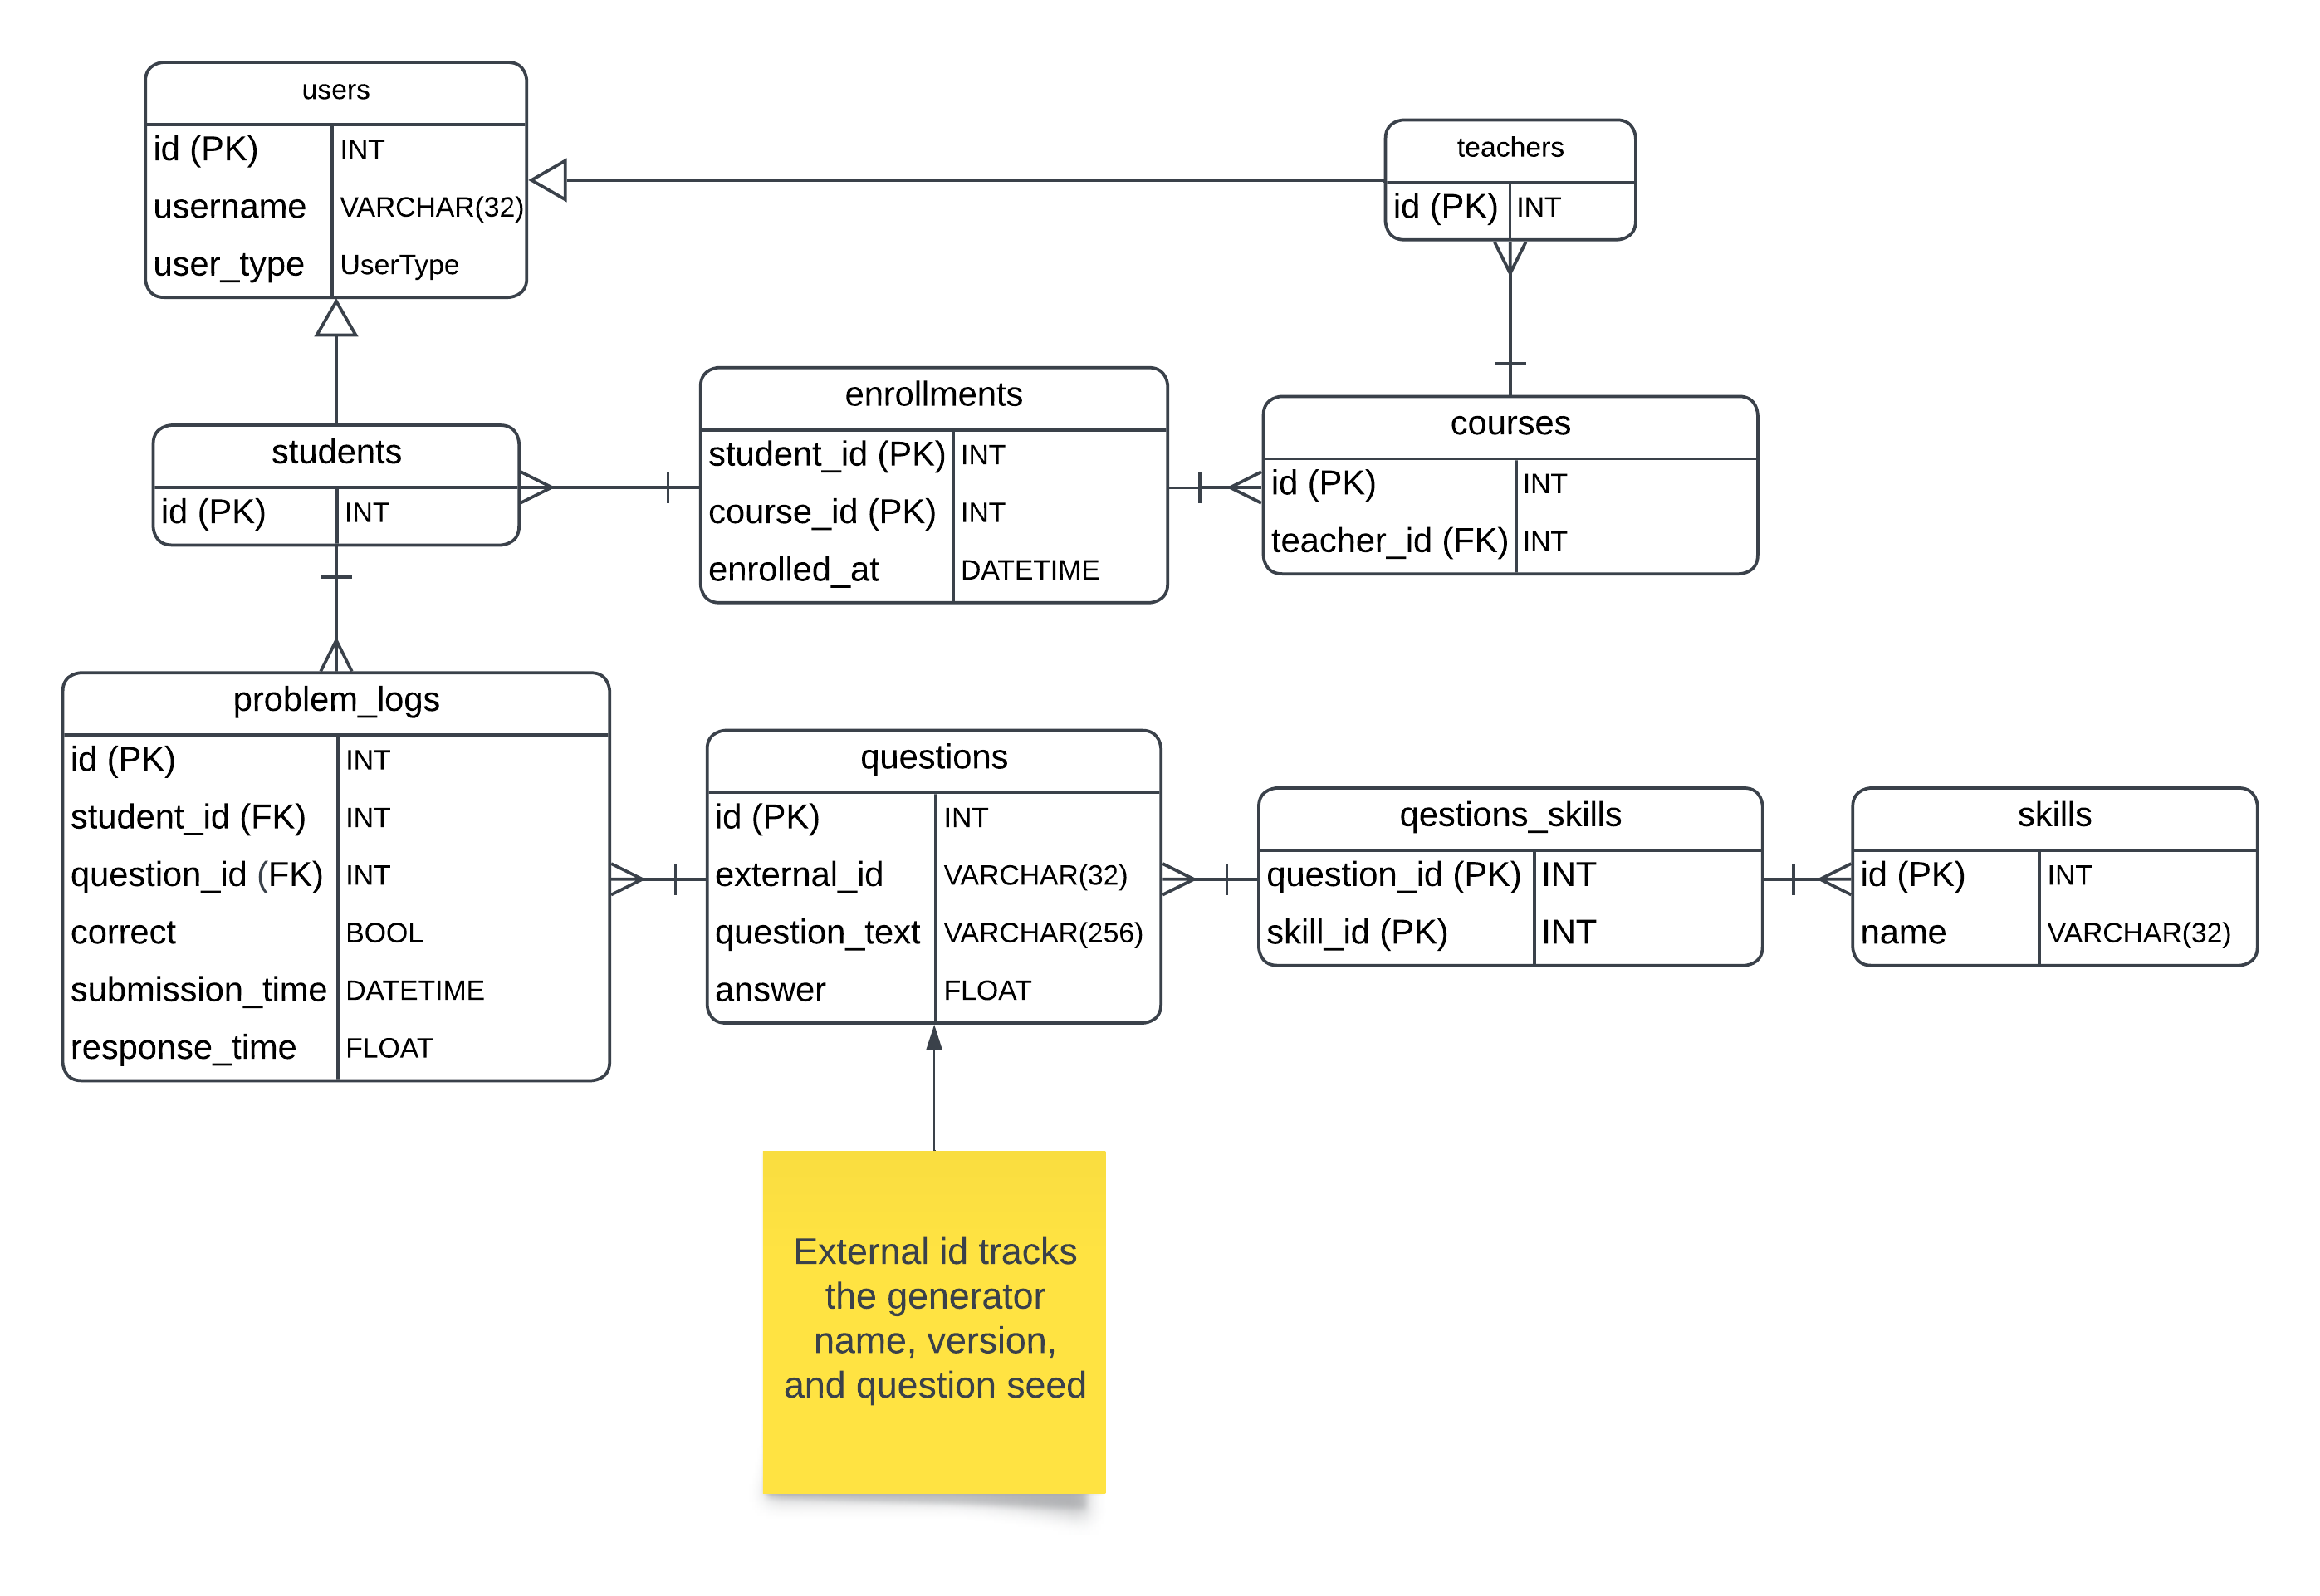
\includegraphics[width=\textwidth]{database_diagram.png}
    \caption{Database diagram}\label{figure:database_diagram}
\end{figure}


\end{document}
